% Options for packages loaded elsewhere
\PassOptionsToPackage{unicode}{hyperref}
\PassOptionsToPackage{hyphens}{url}
%
\documentclass[
]{article}
\usepackage{amsmath,amssymb}
\usepackage{iftex}
\ifPDFTeX
  \usepackage[T1]{fontenc}
  \usepackage[utf8]{inputenc}
  \usepackage{textcomp} % provide euro and other symbols
\else % if luatex or xetex
  \usepackage{unicode-math} % this also loads fontspec
  \defaultfontfeatures{Scale=MatchLowercase}
  \defaultfontfeatures[\rmfamily]{Ligatures=TeX,Scale=1}
\fi
\usepackage{lmodern}
\ifPDFTeX\else
  % xetex/luatex font selection
\fi
% Use upquote if available, for straight quotes in verbatim environments
\IfFileExists{upquote.sty}{\usepackage{upquote}}{}
\IfFileExists{microtype.sty}{% use microtype if available
  \usepackage[]{microtype}
  \UseMicrotypeSet[protrusion]{basicmath} % disable protrusion for tt fonts
}{}
\makeatletter
\@ifundefined{KOMAClassName}{% if non-KOMA class
  \IfFileExists{parskip.sty}{%
    \usepackage{parskip}
  }{% else
    \setlength{\parindent}{0pt}
    \setlength{\parskip}{6pt plus 2pt minus 1pt}}
}{% if KOMA class
  \KOMAoptions{parskip=half}}
\makeatother
\usepackage{xcolor}
\usepackage[margin=1in]{geometry}
\usepackage{color}
\usepackage{fancyvrb}
\newcommand{\VerbBar}{|}
\newcommand{\VERB}{\Verb[commandchars=\\\{\}]}
\DefineVerbatimEnvironment{Highlighting}{Verbatim}{commandchars=\\\{\}}
% Add ',fontsize=\small' for more characters per line
\usepackage{framed}
\definecolor{shadecolor}{RGB}{248,248,248}
\newenvironment{Shaded}{\begin{snugshade}}{\end{snugshade}}
\newcommand{\AlertTok}[1]{\textcolor[rgb]{0.94,0.16,0.16}{#1}}
\newcommand{\AnnotationTok}[1]{\textcolor[rgb]{0.56,0.35,0.01}{\textbf{\textit{#1}}}}
\newcommand{\AttributeTok}[1]{\textcolor[rgb]{0.13,0.29,0.53}{#1}}
\newcommand{\BaseNTok}[1]{\textcolor[rgb]{0.00,0.00,0.81}{#1}}
\newcommand{\BuiltInTok}[1]{#1}
\newcommand{\CharTok}[1]{\textcolor[rgb]{0.31,0.60,0.02}{#1}}
\newcommand{\CommentTok}[1]{\textcolor[rgb]{0.56,0.35,0.01}{\textit{#1}}}
\newcommand{\CommentVarTok}[1]{\textcolor[rgb]{0.56,0.35,0.01}{\textbf{\textit{#1}}}}
\newcommand{\ConstantTok}[1]{\textcolor[rgb]{0.56,0.35,0.01}{#1}}
\newcommand{\ControlFlowTok}[1]{\textcolor[rgb]{0.13,0.29,0.53}{\textbf{#1}}}
\newcommand{\DataTypeTok}[1]{\textcolor[rgb]{0.13,0.29,0.53}{#1}}
\newcommand{\DecValTok}[1]{\textcolor[rgb]{0.00,0.00,0.81}{#1}}
\newcommand{\DocumentationTok}[1]{\textcolor[rgb]{0.56,0.35,0.01}{\textbf{\textit{#1}}}}
\newcommand{\ErrorTok}[1]{\textcolor[rgb]{0.64,0.00,0.00}{\textbf{#1}}}
\newcommand{\ExtensionTok}[1]{#1}
\newcommand{\FloatTok}[1]{\textcolor[rgb]{0.00,0.00,0.81}{#1}}
\newcommand{\FunctionTok}[1]{\textcolor[rgb]{0.13,0.29,0.53}{\textbf{#1}}}
\newcommand{\ImportTok}[1]{#1}
\newcommand{\InformationTok}[1]{\textcolor[rgb]{0.56,0.35,0.01}{\textbf{\textit{#1}}}}
\newcommand{\KeywordTok}[1]{\textcolor[rgb]{0.13,0.29,0.53}{\textbf{#1}}}
\newcommand{\NormalTok}[1]{#1}
\newcommand{\OperatorTok}[1]{\textcolor[rgb]{0.81,0.36,0.00}{\textbf{#1}}}
\newcommand{\OtherTok}[1]{\textcolor[rgb]{0.56,0.35,0.01}{#1}}
\newcommand{\PreprocessorTok}[1]{\textcolor[rgb]{0.56,0.35,0.01}{\textit{#1}}}
\newcommand{\RegionMarkerTok}[1]{#1}
\newcommand{\SpecialCharTok}[1]{\textcolor[rgb]{0.81,0.36,0.00}{\textbf{#1}}}
\newcommand{\SpecialStringTok}[1]{\textcolor[rgb]{0.31,0.60,0.02}{#1}}
\newcommand{\StringTok}[1]{\textcolor[rgb]{0.31,0.60,0.02}{#1}}
\newcommand{\VariableTok}[1]{\textcolor[rgb]{0.00,0.00,0.00}{#1}}
\newcommand{\VerbatimStringTok}[1]{\textcolor[rgb]{0.31,0.60,0.02}{#1}}
\newcommand{\WarningTok}[1]{\textcolor[rgb]{0.56,0.35,0.01}{\textbf{\textit{#1}}}}
\usepackage{graphicx}
\makeatletter
\def\maxwidth{\ifdim\Gin@nat@width>\linewidth\linewidth\else\Gin@nat@width\fi}
\def\maxheight{\ifdim\Gin@nat@height>\textheight\textheight\else\Gin@nat@height\fi}
\makeatother
% Scale images if necessary, so that they will not overflow the page
% margins by default, and it is still possible to overwrite the defaults
% using explicit options in \includegraphics[width, height, ...]{}
\setkeys{Gin}{width=\maxwidth,height=\maxheight,keepaspectratio}
% Set default figure placement to htbp
\makeatletter
\def\fps@figure{htbp}
\makeatother
\setlength{\emergencystretch}{3em} % prevent overfull lines
\providecommand{\tightlist}{%
  \setlength{\itemsep}{0pt}\setlength{\parskip}{0pt}}
\setcounter{secnumdepth}{-\maxdimen} % remove section numbering
\ifLuaTeX
  \usepackage{selnolig}  % disable illegal ligatures
\fi
\usepackage{bookmark}
\IfFileExists{xurl.sty}{\usepackage{xurl}}{} % add URL line breaks if available
\urlstyle{same}
\hypersetup{
  pdftitle={Assessing North Carolina's Aging Population and Affordable Housing Crisis},
  pdfauthor={Ramya Subramanian},
  hidelinks,
  pdfcreator={LaTeX via pandoc}}

\title{Assessing North Carolina's Aging Population and Affordable
Housing Crisis}
\author{Ramya Subramanian}
\date{2025-11-02}

\begin{document}
\maketitle

\begin{Shaded}
\begin{Highlighting}[]
\NormalTok{knitr}\SpecialCharTok{::}\NormalTok{opts\_chunk}\SpecialCharTok{$}\FunctionTok{set}\NormalTok{(}\AttributeTok{echo =} \ConstantTok{TRUE}\NormalTok{)}
\end{Highlighting}
\end{Shaded}

Affordable housing is minimal in many parts of North Carolina.
Specifically, the elderly population are increasingly at risk of
displacement due to being on fixed incomes. I will be examining where
our aging population who are owners and renters of homes are found
across North Carolina and its relationship to median monthly housing
costs in 2023.

Source: \url{https://nciom.org/aging-with-dignity-in-north-carolina/}

\subsubsection{Loading Libraries}\label{loading-libraries}

\begin{Shaded}
\begin{Highlighting}[]
\FunctionTok{library}\NormalTok{(ggplot2)}
\FunctionTok{library}\NormalTok{(tidycensus)}
\FunctionTok{library}\NormalTok{(tmap)}
\FunctionTok{library}\NormalTok{(tmaptools)}
\FunctionTok{library}\NormalTok{(dplyr)        }
\FunctionTok{library}\NormalTok{(sf)      }
\FunctionTok{library}\NormalTok{(RColorBrewer)}
\FunctionTok{library}\NormalTok{(classInt)     }
\FunctionTok{library}\NormalTok{(tidyverse)        }
\FunctionTok{library}\NormalTok{(cartography) }
\FunctionTok{library}\NormalTok{(SpatialPosition)}
\FunctionTok{library}\NormalTok{(maptiles) }
\FunctionTok{library}\NormalTok{(terra)}
\FunctionTok{library}\NormalTok{(potential)}
\end{Highlighting}
\end{Shaded}

\subsubsection{Access API Code and Load Census
Data}\label{access-api-code-and-load-census-data}

\begin{Shaded}
\begin{Highlighting}[]
\CommentTok{\#census\_api\_key("f3d78e8619bc671c28d7a271bf415a2377086d51", install = TRUE)}
\CommentTok{\# Using 2023 census data from American Community Survey 5 Year Data}
\NormalTok{v2023 }\OtherTok{\textless{}{-}} \FunctionTok{load\_variables}\NormalTok{(}\DecValTok{2023}\NormalTok{, }\StringTok{"acs5"}\NormalTok{, }\AttributeTok{cache =} \ConstantTok{FALSE}\NormalTok{)}
\CommentTok{\# North Carolina\textquotesingle{}s Median Monthly Housing Costs and Age 65{-}74 Owners and Renters}
\NormalTok{variables }\OtherTok{\textless{}{-}} \FunctionTok{c}\NormalTok{(}
  \AttributeTok{MedianHouse =} \StringTok{"B25105\_001"}\NormalTok{,}
  \AttributeTok{NCOwner65 =} \StringTok{"B25007\_009"}\NormalTok{,}
  \AttributeTok{NCRenter65 =} \StringTok{"B25007\_019"}
\NormalTok{)}

\NormalTok{NCarolina }\OtherTok{\textless{}{-}} \FunctionTok{get\_acs}\NormalTok{(}\AttributeTok{state =} \StringTok{"NC"}\NormalTok{, }\AttributeTok{geography =} \StringTok{"tract"}\NormalTok{, }\AttributeTok{variables =}\NormalTok{ variables, }\AttributeTok{geometry =} \ConstantTok{TRUE}\NormalTok{, }\AttributeTok{cb =} \ConstantTok{FALSE}\NormalTok{)}
\end{Highlighting}
\end{Shaded}

\subsubsection{Cleaning Data}\label{cleaning-data}

\begin{Shaded}
\begin{Highlighting}[]
\NormalTok{NCarolina1 }\OtherTok{\textless{}{-}}\NormalTok{ NCarolina }\CommentTok{\# easy to make changes without downloading census data multiple times}
\NormalTok{NCarolina1}\SpecialCharTok{$}\NormalTok{variable }\OtherTok{\textless{}{-}} \FunctionTok{as.factor}\NormalTok{(NCarolina1}\SpecialCharTok{$}\NormalTok{variable) }\CommentTok{\# make variables factors}

\CommentTok{\#Group the variables by county tract and make each variable its own column}
\NormalTok{NCarolina1\_wide }\OtherTok{\textless{}{-}}\NormalTok{ NCarolina1 }\SpecialCharTok{\%\textgreater{}\%}
  \FunctionTok{group\_by}\NormalTok{(NAME, variable) }\SpecialCharTok{\%\textgreater{}\%}
  \FunctionTok{summarise}\NormalTok{(}
    \AttributeTok{estimate =} \FunctionTok{mean}\NormalTok{(estimate, }\AttributeTok{na.rm =} \ConstantTok{TRUE}\NormalTok{),}
    \AttributeTok{.groups =} \StringTok{"drop"}
\NormalTok{  ) }\SpecialCharTok{\%\textgreater{}\%}
  \FunctionTok{pivot\_wider}\NormalTok{(}
    \AttributeTok{names\_from =}\NormalTok{ variable,}
    \AttributeTok{values\_from =}\NormalTok{ estimate,}
    \AttributeTok{values\_fn =}\NormalTok{ mean,        }\CommentTok{\# or first, if each combo is unique}
    \AttributeTok{values\_fill =} \DecValTok{0}
\NormalTok{  )}
\CommentTok{\# Split county tract variable to access just county name}
\NormalTok{NCarolina1\_wide }\OtherTok{\textless{}{-}}\NormalTok{ NCarolina1\_wide }\SpecialCharTok{\%\textgreater{}\%}
  \FunctionTok{mutate}\NormalTok{(}
    \AttributeTok{County =} \FunctionTok{trimws}\NormalTok{(}\FunctionTok{strsplit}\NormalTok{(NAME, }\StringTok{";"}\NormalTok{) }\SpecialCharTok{\%\textgreater{}\%} \FunctionTok{sapply}\NormalTok{(}\StringTok{\textasciigrave{}}\AttributeTok{[}\StringTok{\textasciigrave{}}\NormalTok{, }\DecValTok{2}\NormalTok{))  }\CommentTok{\# get 2nd item}
\NormalTok{  )}
\CommentTok{\# Grouping Tracts into County}
\NormalTok{NCarolina\_county }\OtherTok{\textless{}{-}}\NormalTok{ NCarolina1\_wide }\SpecialCharTok{\%\textgreater{}\%}
  \FunctionTok{group\_by}\NormalTok{(County) }\SpecialCharTok{\%\textgreater{}\%}
  \FunctionTok{summarize}\NormalTok{(}
    \AttributeTok{MedianHouse =} \FunctionTok{mean}\NormalTok{(MedianHouse, }\AttributeTok{na.rm =} \ConstantTok{TRUE}\NormalTok{),}
    \AttributeTok{NCOwner65 =} \FunctionTok{sum}\NormalTok{(NCOwner65, }\AttributeTok{na.rm =} \ConstantTok{TRUE}\NormalTok{),}
    \AttributeTok{NCRenter65 =} \FunctionTok{sum}\NormalTok{(NCRenter65, }\AttributeTok{na.rm =} \ConstantTok{TRUE}\NormalTok{),}
    \AttributeTok{geometry =} \FunctionTok{st\_union}\NormalTok{(geometry),}
    \AttributeTok{.groups =} \StringTok{"drop"}
\NormalTok{  ) }\SpecialCharTok{\%\textgreater{}\%}
  \FunctionTok{st\_as\_sf}\NormalTok{() }\CommentTok{\#make into spatial feature}

\FunctionTok{head}\NormalTok{(NCarolina\_county)}
\end{Highlighting}
\end{Shaded}

\begin{verbatim}
## Simple feature collection with 6 features and 4 fields
## Geometry type: POLYGON
## Dimension:     XY
## Bounding box:  xmin: -82.08108 ymin: 34.80671 xmax: -79.2366 ymax: 36.58814
## Geodetic CRS:  NAD83
## # A tibble: 6 x 5
##   County           MedianHouse NCOwner65 NCRenter65                     geometry
##   <chr>                  <dbl>     <dbl>      <dbl>                <POLYGON [°]>
## 1 Alamance County         995.      8707       2208 ((-79.39252 35.8438, -79.38~
## 2 Alexander County        645       2573        273 ((-81.02985 35.89012, -81.0~
## 3 Alleghany County        741       1138        105 ((-81.15358 36.57008, -81.1~
## 4 Anson County            795.      1401        321 ((-80.17853 35.14996, -80.1~
## 5 Ashe County             725.      2011        340 ((-81.74193 36.41115, -81.7~
## 6 Avery County            673.      1334        173 ((-81.97563 36.20508, -81.9~
\end{verbatim}

\subsubsection{Visual 1: Median Monthly Housing Costs by County in North
Carolina}\label{visual-1-median-monthly-housing-costs-by-county-in-north-carolina}

\begin{Shaded}
\begin{Highlighting}[]
\FunctionTok{tm\_shape}\NormalTok{(NCarolina\_county) }\SpecialCharTok{+}
  \FunctionTok{tm\_polygons}\NormalTok{(}
    \AttributeTok{col =} \StringTok{"MedianHouse"}\NormalTok{,}
    \AttributeTok{palette =} \StringTok{"{-}RdYlGn"}\NormalTok{,}
    \AttributeTok{style =} \StringTok{"quantile"}\NormalTok{,}
    \AttributeTok{border.col =} \ConstantTok{NA}\NormalTok{,}
    \AttributeTok{title =} \StringTok{"Median Housing Costs ($)"}
\NormalTok{  ) }\SpecialCharTok{+}
  \FunctionTok{tm\_layout}\NormalTok{(}
    \AttributeTok{legend.outside =} \ConstantTok{TRUE}\NormalTok{,}
    \AttributeTok{legend.outside.position =} \StringTok{"right"}\NormalTok{,}
    \AttributeTok{main.title =} \StringTok{"North Carolina Median Housing Costs Per County in 2023"}\NormalTok{,}
    \AttributeTok{main.title.size =} \FloatTok{1.2}\NormalTok{,}
    \AttributeTok{main.title.fontface =} \StringTok{"bold"}
\NormalTok{  ) }\SpecialCharTok{+}
  \FunctionTok{tm\_compass}\NormalTok{(}\AttributeTok{position =} \FunctionTok{c}\NormalTok{(}\StringTok{"left"}\NormalTok{, }\StringTok{"top"}\NormalTok{), }\AttributeTok{size =} \FloatTok{1.5}\NormalTok{) }\SpecialCharTok{+}
  \FunctionTok{tm\_scale\_bar}\NormalTok{(}\AttributeTok{position =} \FunctionTok{c}\NormalTok{(}\StringTok{"left"}\NormalTok{, }\StringTok{"bottom"}\NormalTok{))}
\end{Highlighting}
\end{Shaded}

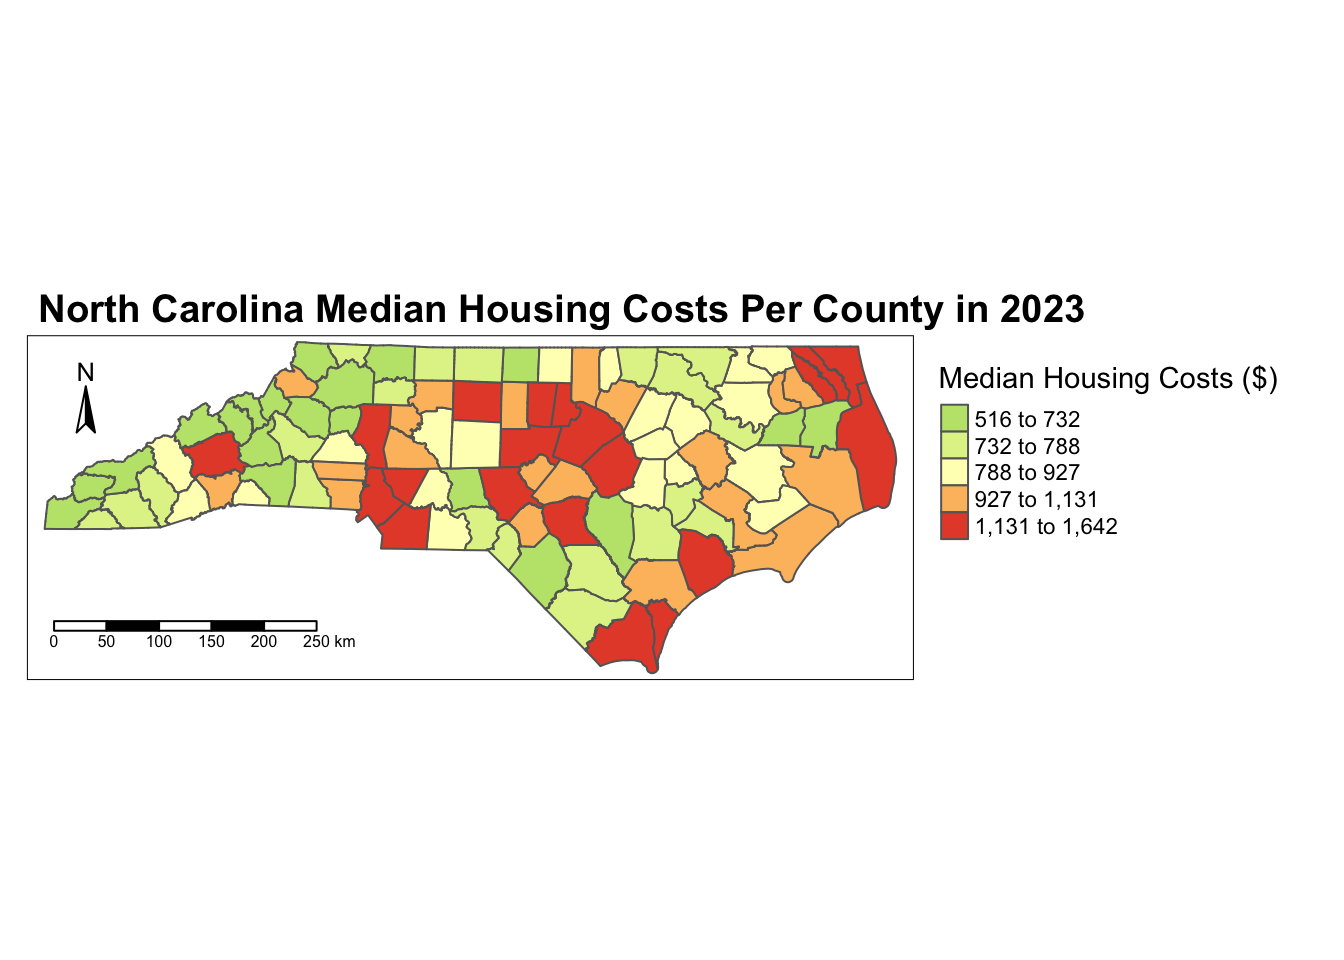
\includegraphics{AdvGeovis_Lab1_files/figure-latex/unnamed-chunk-4-1.pdf}

From this visualization, we can see the median housing costs are
generally higher on mid-east counties of the state.

\subsubsection{Visual 2: Median Housing Costs with 65-74 Homeowner
Distribution}\label{visual-2-median-housing-costs-with-65-74-homeowner-distribution}

\begin{Shaded}
\begin{Highlighting}[]
\CommentTok{\# Centroid for the proportional symbol}
\NormalTok{NCarolina\_centroids }\OtherTok{\textless{}{-}} \FunctionTok{st\_centroid}\NormalTok{(NCarolina\_county)}
\end{Highlighting}
\end{Shaded}

\begin{verbatim}
## Warning: st_centroid assumes attributes are constant over geometries
\end{verbatim}

\begin{Shaded}
\begin{Highlighting}[]
\FunctionTok{tm\_shape}\NormalTok{(NCarolina\_county) }\SpecialCharTok{+} \CommentTok{\#Mean Housing Chloropleth}
  \FunctionTok{tm\_polygons}\NormalTok{(}
    \AttributeTok{col =} \StringTok{"MedianHouse"}\NormalTok{,}
    \AttributeTok{palette =} \StringTok{"{-}RdYlGn"}\NormalTok{,}
    \AttributeTok{style =} \StringTok{"quantile"}\NormalTok{,}
    \AttributeTok{border.col =} \ConstantTok{NA}\NormalTok{,}
    \AttributeTok{title =} \StringTok{"Median Housing Costs ($)"}
\NormalTok{  ) }\SpecialCharTok{+}
  \FunctionTok{tm\_shape}\NormalTok{(NCarolina\_centroids) }\SpecialCharTok{+} \CommentTok{\#Proportional Symbol}
  \FunctionTok{tm\_symbols}\NormalTok{(}
    \AttributeTok{size =} \StringTok{"NCOwner65"}\NormalTok{,   }
    \AttributeTok{col =} \StringTok{"black"}\NormalTok{,            }
    \AttributeTok{alpha =} \FloatTok{0.6}\NormalTok{,}
    \AttributeTok{scale =} \FloatTok{1.5}\NormalTok{,}
    \AttributeTok{border.col =} \StringTok{"white"}\NormalTok{,}
    \AttributeTok{legend.size.show =} \ConstantTok{TRUE}\NormalTok{,}
    \AttributeTok{title.size =} \StringTok{"\# of Home Owners Aged 65{-}74"}
\NormalTok{  ) }\SpecialCharTok{+}
  \FunctionTok{tm\_layout}\NormalTok{(}
    \AttributeTok{main.title =} \StringTok{"North Carolina Elderly Adult Homeownership }\SpecialCharTok{\textbackslash{}n}\StringTok{\& Housing Costs in 2023"}\NormalTok{,}
    \AttributeTok{main.title.position =} \FunctionTok{c}\NormalTok{(}\StringTok{"center"}\NormalTok{, }\StringTok{"top"}\NormalTok{),}
    \AttributeTok{main.title.size =} \FloatTok{1.2}\NormalTok{,}
    \AttributeTok{main.title.fontface =} \StringTok{"bold"}\NormalTok{,}
    \AttributeTok{outer.margins =} \FunctionTok{c}\NormalTok{(}\FloatTok{0.1}\NormalTok{, }\FloatTok{0.02}\NormalTok{, }\FloatTok{0.02}\NormalTok{, }\FloatTok{0.02}\NormalTok{),}
    \AttributeTok{legend.text.size =} \FloatTok{0.61}\NormalTok{,}
    \AttributeTok{legend.outside =} \ConstantTok{TRUE}\NormalTok{,}
    \AttributeTok{legend.outside.position =} \StringTok{"left"}
\NormalTok{  ) }\SpecialCharTok{+}
    \FunctionTok{tm\_compass}\NormalTok{(}\AttributeTok{position =} \FunctionTok{c}\NormalTok{(}\StringTok{"left"}\NormalTok{, }\StringTok{"top"}\NormalTok{), }\AttributeTok{size =} \FloatTok{1.5}\NormalTok{) }\SpecialCharTok{+}
    \FunctionTok{tm\_scale\_bar}\NormalTok{(}\AttributeTok{position =} \FunctionTok{c}\NormalTok{(}\StringTok{"left"}\NormalTok{, }\StringTok{"bottom"}\NormalTok{))}
\end{Highlighting}
\end{Shaded}

\begin{verbatim}
## Legend labels were too wide. Therefore, legend.text.size has been set to 0.6. Increase legend.width (argument of tm_layout) to make the legend wider and therefore the labels larger.
\end{verbatim}

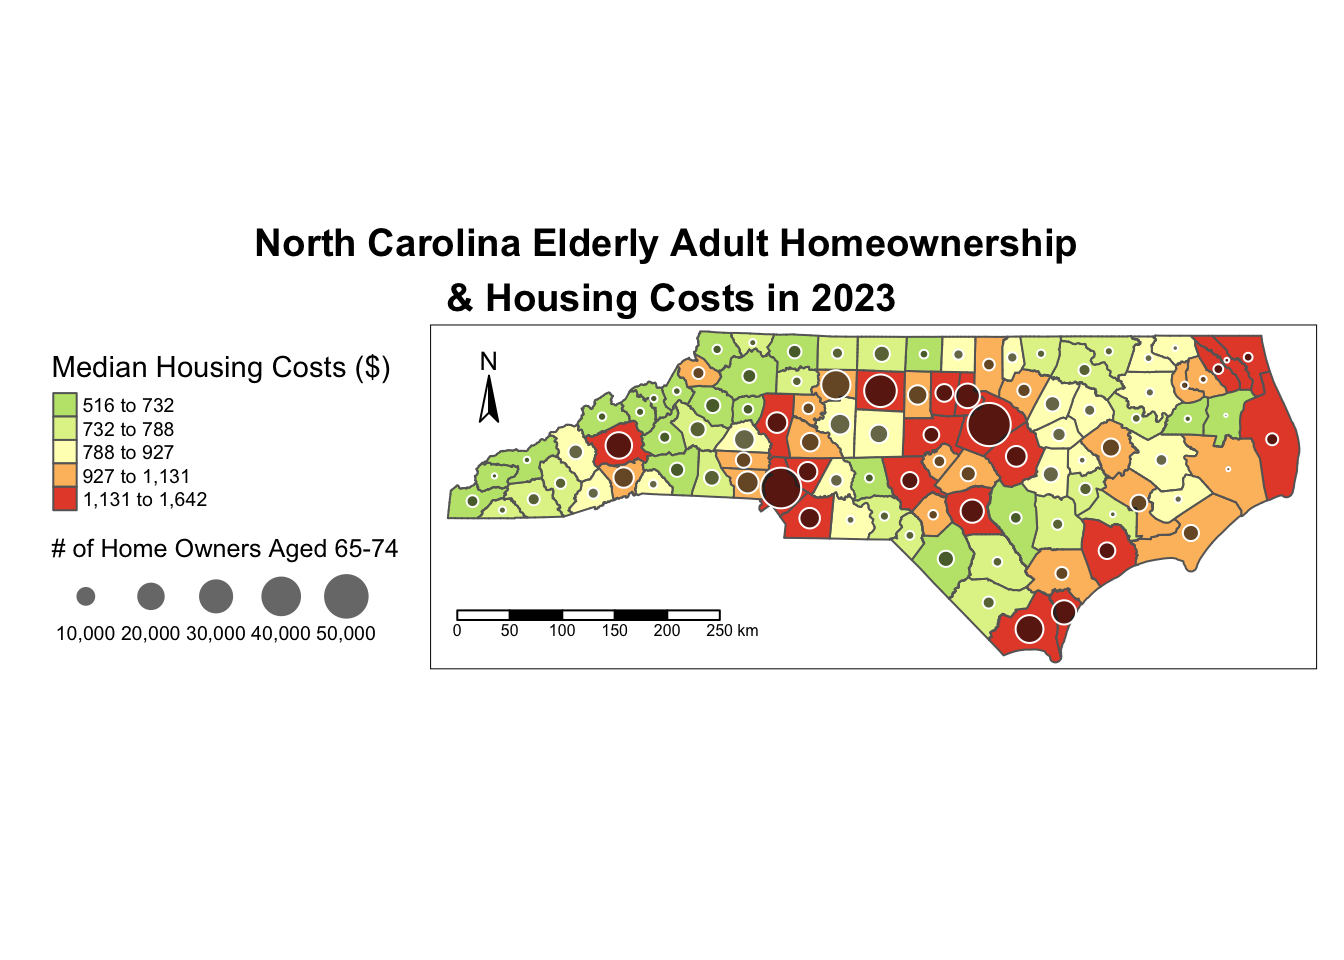
\includegraphics{AdvGeovis_Lab1_files/figure-latex/unnamed-chunk-5-1.pdf}

In the center of the state, the counties that are red with high median
housing costs and high number of older home owners may face a higher
risk of housing crisis. The west side of the state seems to have both
less housing costs and elderly home owners.

\subsubsection{Visual 3: Ratio of Owners verus Renters Aged
65-74}\label{visual-3-ratio-of-owners-verus-renters-aged-65-74}

\begin{Shaded}
\begin{Highlighting}[]
\CommentTok{\# Create a logical flag for top 25\% renter tracts}
\NormalTok{NCarolina\_county }\OtherTok{\textless{}{-}}\NormalTok{ NCarolina\_county }\SpecialCharTok{\%\textgreater{}\%}
  \FunctionTok{mutate}\NormalTok{(}
    \AttributeTok{OwnerRenterRatio =}\NormalTok{ NCOwner65 }\SpecialCharTok{/}\NormalTok{ NCRenter65}
\NormalTok{  )}

\FunctionTok{tm\_shape}\NormalTok{(NCarolina\_county) }\SpecialCharTok{+}
  \FunctionTok{tm\_polygons}\NormalTok{(}
    \AttributeTok{col =} \StringTok{"OwnerRenterRatio"}\NormalTok{,}
    \AttributeTok{palette =} \StringTok{"RdBu"}\NormalTok{,         }\CommentTok{\# Red = more renters, Blue = more owners}
    \AttributeTok{style =} \StringTok{"quantile"}\NormalTok{,       }\CommentTok{\# Try "pretty" or "jenks" if it looks off}
    \AttributeTok{border.col =} \ConstantTok{NA}\NormalTok{,}
    \AttributeTok{title =} \StringTok{"Owner{-}to{-}Renter Ratio"}
\NormalTok{  ) }\SpecialCharTok{+}
  \FunctionTok{tm\_layout}\NormalTok{(}
    \AttributeTok{main.title =} \StringTok{"North Carolina Ratio of Owners to Renters }\SpecialCharTok{\textbackslash{}n}\StringTok{Aged 65{-}74 by County in 2023"}\NormalTok{,}
    \AttributeTok{main.title.position =} \FunctionTok{c}\NormalTok{(}\StringTok{"center"}\NormalTok{, }\StringTok{"top"}\NormalTok{),}
    \AttributeTok{main.title.size =} \FloatTok{1.2}\NormalTok{,}
    \AttributeTok{main.title.fontface =} \StringTok{"bold"}\NormalTok{,}
    \AttributeTok{outer.margins =} \FunctionTok{c}\NormalTok{(}\FloatTok{0.1}\NormalTok{, }\FloatTok{0.02}\NormalTok{, }\FloatTok{0.02}\NormalTok{, }\FloatTok{0.02}\NormalTok{),}
    \AttributeTok{legend.outside =} \ConstantTok{TRUE}\NormalTok{,}
    \AttributeTok{legend.outside.position =} \StringTok{"right"}
\NormalTok{  ) }\SpecialCharTok{+}
    \FunctionTok{tm\_compass}\NormalTok{(}\AttributeTok{position =} \FunctionTok{c}\NormalTok{(}\StringTok{"left"}\NormalTok{, }\StringTok{"top"}\NormalTok{), }\AttributeTok{size =} \FloatTok{1.5}\NormalTok{) }\SpecialCharTok{+}
    \FunctionTok{tm\_scale\_bar}\NormalTok{(}\AttributeTok{position =} \FunctionTok{c}\NormalTok{(}\StringTok{"left"}\NormalTok{, }\StringTok{"bottom"}\NormalTok{))}
\end{Highlighting}
\end{Shaded}

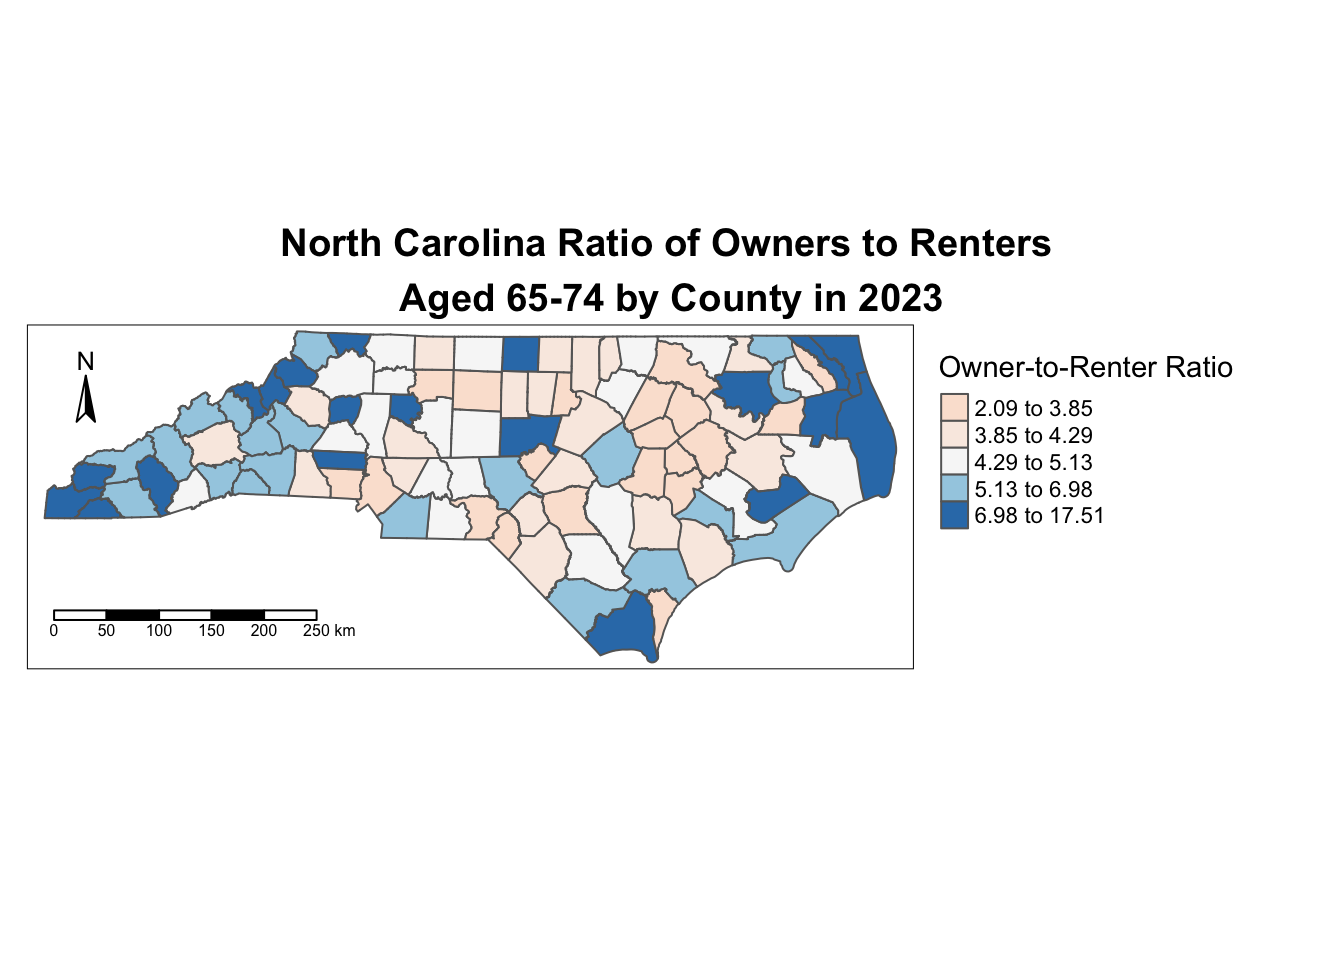
\includegraphics{AdvGeovis_Lab1_files/figure-latex/unnamed-chunk-6-1.pdf}

It seems there are more elderly owners than renters in the areas on the
edges of the states while the center is more renter heavier.
Interestingly, the center of the state is where we saw the higher
housing costs. This may explain why we find more elderly renters and
more struggling elderly owners in these counties.

\subsubsection{Assignment Questions}\label{assignment-questions}

\textbf{1. Discuss the advantages and challenges associated with an open
data science approach. Provide an example based on this week's reading.
(1-2 paragraphs)}

An advantage of the open data science approach is the increase in
innovation and efficiency when data sets are able to be reused for new
projects by new people. Kitchin (2013) discusses how useful big data has
become in supplying detailed and low-cost data that can help promote the
value of geography to a wider audience like Obama's team collecting
voter data before the election. With all this new data accessible,
having an open data science approach can make big data even more
powerful. This also helps data creators to reach broader audiences when
data is openly shared as their information is more accessible. A
challenge with the open data science approach is data quality issues.
Kitchin (2013) explains how big data can make it difficult to extract
useful and valid information from the data deluge of vast information.
When there is so much data, it can be hard to discern what data is
actually useful which is common in open data science approaches that
leave you with too much information.

\textbf{2. Create a markdown document that showcases an analysis of this
week's data or any other dataset of your choice. Include descriptive
text that explains your analysis, and incorporate figures and
geovisualizations.Include 1 chart and 1 map. Structure and explain your
analysis with text, headings, highlights, images and other markdown
basics.}

For my maps, I chose to answer the research question: how do the mean
housing costs and the aging population of home owners and renters in
North Carolina inform us of the rising affordable housing crisis. I
created a chloropleth map visualizing the mean housing costs in all the
counties of North Carolina to get an understanding of which areas have
higher housing costs. For the next map, I chose to create a proportional
symbol map layered on top of the chloropleth map I previously made to
showcase the number of aged 65-74 homeowners for each state in
comparison to the mean housing cost level of that county. The specific
steps I took to mitigate bias is I chose to classify the data by
quantiles to ensure the data was represented as accurately as possible
while differentiating between classes. The final map I created is a
ratio of owners to renters aged 65-74 to visually understand what type
of elderly population is more prevalent when concerned with hosuing
costs in North Carolina counties. As a chloropleth map, this can be
useful to easily point out the counties with more owners compared to
renters to better inform the other maps about where housing costs being
high is more of a problem. I minimized bias by calculating a ratio
versus simply showing owners versus renters to normalize the data.

\end{document}
